\section{补充推导}
\label{app:proofs}
\paragraph{实际归一化。}
令$m_t\in\{0,1\}$为最终actor mask，$n_b=\sum_{t\in b}m_t$、$N=\sum_t m_t$、$\eta=10^{-8}$。空块取$\bar a_b=0$。
代码用分数block mask最小化负的裁剪代理目标：
\begin{equation}
 L_{\mathrm{blk}}=-\frac{\sum_b(n_b/k)\mathcal C(R_b,\bar a_b)}{N/k+\eta}
 =-\frac{\sum_b n_b\mathcal C(R_b,\bar a_b)}{N+k\eta}.
\end{equation}
token分母为$N+\eta$。聚合前先将无效位置置零，不删除mask空洞，不把相邻token移动到不同block。
空块和padding权重均为零。
actor micro-batch=1时，更新平均各条响应独立归一化的loss；响应长度不同时，它不是整个batch的全局token均值。
因此仅凭\texttt{token-mean}配置名，不能认定实现了DAPO使用的全局加权\citep{dapo}。

\paragraph{裁剪约定。}
取ratio下限$d=0.8$、上限$u=1.2$，定义$s(r,a)=\min\{ra,\clip(r,d,u)a\}$，继承目标为
\begin{equation}
 \mathcal C(r,a)=\begin{cases}\max\{s(r,a),3a\},&a<0,\\s(r,a),&a\ge0.\end{cases}
\end{equation}
这是普通PPO裁剪加负advantage dual-clip。先计算block ratio，再应用此操作。
梯度范数裁剪到1是另一个独立优化器操作；两者均不保证未来所有policy ratio或teacher KL始终处于指定范围。

\paragraph{一阶导数与合成检查。}
在梯度生效分支上，对有效$t\in b$，关于当前采样log probability的导数为
\begin{equation}
 \frac{\partial L_{\mathrm{blk}}}{\partial\log p_\theta(y_t\mid h_t)}
 =-\frac{n_b\bar a_bR_b}{N+k\eta},\qquad
 \frac{\partial L_{\mathrm{tok}}}{\partial\log p_\theta(y_t\mid h_t)}
 =-\frac{a_tr_t}{N+\eta}.
\end{equation}
ratio=1时，在$\eta=0$的理想化下，任意advantage的两种策略loss数值一致，但导数不一定一致。
5个token均有$a_t=1$时，token导数均为$-1/5$，Block3则为$(-3/5,-3/5,-3/5,-2/5,-2/5)$。
当$(a_1,a_2,a_3)=(1,-1,1)$时，token导数为$(-1/3,1/3,-1/3)$，block导数为$(-1/3,-1/3,-1/3)$。
这些是合成导数示例，不是真实参数更新幅度的估计。

\paragraph{受限的信用范围解释。}
假设固定horizon $T$、确定性连续划分、无mask或截断，学生支撑集局部不依赖参数、固定教师$q$在其上为正，
从完整当前学生分布$p_\theta$采样，log probability可微且允许交换微分与期望。
定义$c_t=\log p_\theta(y_t\mid h_t)-\log q(y_t\mid h_t)$和
$g_t=\nabla\log p_\theta(y_t\mid h_t)$，则
\begin{align}
 \nabla\KL(P_\theta\Vert Q)
 &=\E\left[\left(\sum_t c_t\right)\left(\sum_t g_t\right)\right] \\
 &=\E\left[\sum_t g_t\sum_{u=t}^{T}c_u\right].
 \label{eq:fullcredit}
\end{align}
log-density本身导数的期望为零。$u<t$时，$c_u$在$h_t$处已知，且$\E[g_t\mid h_t]=0$，所以过去项在期望中消失。
定义$H_{\mathrm{blk}}=\sum_b(\sum_{u\in b}c_u)(\sum_{t\in b}g_t)$和$H_{\mathrm{seq}}=(\sum_u c_u)(\sum_t g_t)$。
对旧策略处未裁剪的block估计量应用同一推导，得到
\begin{equation}
 \E H_{\mathrm{blk}}=\E\left[\sum_t g_t\sum_{u=t}^{e(t)}c_u\right],\qquad
 \E(H_{\mathrm{seq}}-H_{\mathrm{blk}})=\E\left[\sum_t g_t\sum_{u>e(t)}c_u\right],
 \label{eq:horizon}
\end{equation}
其中$e(t)$为token $t$所在block的末端。
相对完全局部的token反馈，block聚合可以恢复块内未来信用，但忽略跨块边界的信用。
因此不能把全部交叉项都称为有害泄漏。被忽略向量可能互相抵消，增大block不一定单调减小偏差。
MiniLLM已考虑未来奖励，此解释不是首次提出蒸馏的时间信用分配\citep{minillm}。

上述恒等式不证明实际loss精确优化完整序列KL。top-$p$会使真实采样分布不同于被评分的学生分布；
masked位置的ratio乘积一般不是block边缘似然比；裁剪和冻结旧策略target会改变远离旧策略后的目标；
随机响应长度归一化又引入对未来动作的依赖。
因此这些是有明确假设的解释性理想化，而非对实际实验的保证。

\paragraph{平均误差分解。}
由$a=\mu+\varepsilon$及$\E\varepsilon=0$，展开$Wa-\mu=(W-I)\mu+W\varepsilon$。
交叉项期望为零，且$\E\varepsilon^\top W^\top W\varepsilon=\operatorname{tr}(W\Sigma W^\top)$，即得式\ref{eq:mse}。
独立同方差噪声且$k$个token具有恒定信号时，平均噪声方差为$k\sigma^2/k^2=\sigma^2/k$。
对无噪声确定性信号$(2,-1,2)$，原始估计误差为零，全部替换为均值1会产生平方误差6。
它反驳的是无条件的信号估计收益，并不意味着教师每token ratio总是正确的任务信用信号。

\paragraph{滑动分区能消除哪一种随机性。}
设$X$包含共同参数、已收集batch、mask、冻结target及其他前向随机性。
令$L_r(X)$为offset $r\in\{0,1,2\}$各自完成裁剪和归一后的loss，$G_r(X)=\nabla_\theta L_r(X)$。
对条件均匀的随机offset $U$，实现中的phase平均满足
\begin{equation}
 G_{\mathrm{slide}}(X)=\frac13\sum_{r=0}^2G_r(X)=\E[G_U(X)\mid X].
\end{equation}
在二阶矩有限且$X$分布相同的前提下，全协方差公式给出
\begin{equation}
 \Cov(G_U)-\Cov(G_{\mathrm{slide}})=\E_X[\Cov(G_U\mid X)]\succeq0.
 \label{eq:phasecov}
\end{equation}
它消除了共同状态条件下由offset随机选择引入的方差，不是Sliding3与固定Block3的比较。
PPO裁剪可以处于激活状态，因为它已包含在每个$L_r$内部；之后的梯度范数裁剪和Adam是非线性操作，不在此恒等式内。
不同训练历史会诱导不同的$X$分布，所以该式不是历史运行的性能保证，也不代表一个固定RNG seed的轨迹精确实现了期望。
平均各自loss也不等于先平均advantage再裁剪一次。

当$N>0$且phase-zero分区匹配时，含partial tail的旧实现满足$L_{\mathrm{hist}}=N L_0/(N+k\eta)$。
由于收集到的mask被冻结，梯度也满足相同比例。$\eta=0$时两者归一完全等价。
前置padding或mask空洞可能使分区匹配前提失效；即便理想表达式相同，浮点操作顺序也可能带来微小数值差别。

\section{配置与数据来源}
\label{app:config}
\paragraph{最新模型身份。}
原始学生为从ModelScope获取的\texttt{Qwen/Qwen3-4B-Base}，revision为
\texttt{bbd6fc8d23e8788d987b7b970cbb7bd31c826e38}。
公开教师保留的modelcard标识为\texttt{lllyx/Qwen3-4B-Base-GRPO}，由Rethinking OPD\citep{rethinking}配套发布。
原仓库现重定向至\href{https://huggingface.co/Thinking-Space/Qwen3-4B-Base-GRPO}{\texttt{Thinking-Space/Qwen3-4B-Base-GRPO}}。
它是研究者发布的GRPO checkpoint，不是Qwen官方指令模型，也不是本项目私有训练模型。
下载缓存记录revision为\texttt{1f3b2966edfb75f2f98a00617588c1f748088422}，两个权重文件的ETag与保留的资产hash相符。
modelcard描述其在DAPO-Math-17k-Processed上进行了GRPO；这一上游教师训练不同于本文学生的200步OPD。

\begin{table}[h]
\caption{最新4B completion对照的共享配置。训练rollout推理与完整评测的部分差异是有意设置，且两组一致。}
\centering\small
\begin{tabular}{@{}p{2.5in}p{2.65in}@{}}
\toprule
设置 & 数值 \\
\midrule
训练seed / 数据seed & 21 / 21 \\
更新步数 / 每步prompt / 每题采样 & 200 / 4 / 8 \\
PPO mini-batch / epochs & 32条响应 / 1 \\
Actor / rollout-logprob / 教师micro-batch & 每GPU 1 / 4 / 1 \\
优化器 / 学习率 & AdamW / $2\times10^{-6}$ \\
Adam betas / epsilon / weight decay & $(0.9,0.999)$ / $10^{-8}$ / 0.01 \\
学习率调度 / warmup & 恒定 / warmup比例0 \\
梯度范数裁剪 & 1.0 \\
PPO下/上裁剪 / dual clip & 0.2 / 0.2 / 3.0 \\
显式熵项 / 额外KL损失 & 0 / 关闭 \\
Outcome reward / OPD未来return权重 & 0 / 0 \\
教师target log-ratio裁剪 & 关闭 \\
特殊token OPD mask & 关闭；保留上游response mask \\
输入 / 响应token上限 & 2,048 / 16,384 \\
Temperature / top-$p$ / top-$k$ & 1.0 / 0.9 / 不限制 \\
训练rollout / 评测显存比例 & 0.6 / 0.9 \\
训练最大批量rollout token & 18,432 \\
硬件 / 张量并行度 & 4张A100-80GB / 1 \\
训练参数 / 优化器offload & 开启 / 开启 \\
梯度检查点 & 开启 \\
权重保存step / checkpoint删除 & 50、100、150、200 / 无 \\
诊断频率 / top-$k$ / 位置bin & 每次更新 / 16 / 128 token \\
Block符号阈值 & $10^{-4}$ \\
\bottomrule
\end{tabular}
\end{table}

\paragraph{精确completion提示与停止设置。}
4B Base的训练与评测使用同一completion函数，不含ChatML：
\begin{quote}\small
\texttt{[question]}\\
\texttt{Please solve the problem step by step and put the final answer in}\ \verb|\boxed{}.|\\
\texttt{Solution:}
\end{quote}
各部分之间保留空行，\texttt{Solution:}后保留末尾换行。
显式关闭thinking，但允许普通逐步推理文本。EOS为151643，无额外stop-token ID。
合并checkpoint后检查实际输入token ID。评测使用四个独立TP=1 worker，显存比例0.9，
区别于训练rollout的0.6。CPU合并不改动源训练权重。
原始响应、输入token、请求seed和引擎停止原因均保留。

\paragraph{实际batch与seed。}
数据batch沿用冻结的seed-21 loader。成对验收比较采集后真实source与prompt身份；
若两组以不同方式消耗RNG，仅seed标签相同并不足够。
最新请求seed通过包含step和sample身份的稳定SHA-256规则派生，记录响应本身不会额外消耗训练RNG。
同题8个请求具有不同seed身份。历史固定请求seed实验在附录\ref{app:history}中独立标注。
run card保留了独立window-seed，但它不影响fixed-block组。

\paragraph{训练池。}
直接读取保留parquet可验证题答序列按17,917行周期重复100次。
未经额外Unicode或数学规范化时，有17,237个唯一原始题面字符串、17,249个唯一原始题答组合。
这些是精确字符串计数，不是语义去重。原始展开命令与上游数据集revision未能恢复。
保留文件的SHA-256前缀为\texttt{cf359f257a320aecb}，内部manifest保留完整hash。
哈希检查不证明完整的训练/测试语义去污染。
两种方法使用相同保留数据池，而非各自重新下载当前名称相同但版本可能不同的数据集。

\paragraph{评测文件与判分。}
MATH500使用\texttt{HuggingFaceH4/MATH-500}的test文件，来自MATH和PRM800K评测谱系\citep{math,prm800k}。
AIME24由\texttt{BytedTsinghua-SIA/AIME-2024}转换。
AIME25与AMC23来自公开OPD仓库中保留的对应test parquet，题数分别为30和83；
尤其不能将83题AMC23无说明地视为其他论文的40题子集。
转换后JSONL的hash前缀为：MATH500 \texttt{cc164b47b60771ee}，AIME24 \texttt{6aee5ed24b811ebc}，
AIME25 \texttt{daedf1e406b9d73c}，AMC23 \texttt{a07c52c0098a536a}。

两组使用同一历史external grader，SHA-256前缀为\texttt{04f7a0328be18409}。
每题保留8次独立seed生成。每个完成checkpoint检查预期题目身份、响应数量、原始输出归档，
以及summary与逐条判分的一致性。
这验证评测契约，不证明符号grader在逻辑上绝不会判错。
grader异常或无法解析答案不应被重新解释为已知数学正确。
缺失boxed标记与引擎length停止始终独立报告。

保留转换器的公开默认输入是 \texttt{BytedTsinghua-SIA/DAPO-Math-17k} 中的 \texttt{data/dapo-math-17k.parquet}。但历史 manifest 记录的是复制而来的已转换 parquet，没有原始 Hub revision 或创建100倍展开的命令。当前转换器默认去重会改变该训练池，不能将当前默认值当成精确的历史预处理方案。

\paragraph{回溯性字符串重叠审计。}
比较原始题面字段后，MATH500的500题中有2题与保留训练池完全相同。
将Unicode空白折叠为单个空格、移除首尾空白并进行Unicode casefold后，共有4题匹配（包含前述2题）。
该规范化不改写数学或LaTeX。精确匹配的测试索引为80、276；仅规范化后新增的索引为285、412，
均是保留MATH500产物的零起始索引。AIME24、AIME25和AMC23在两种规则下均为零。
审计依赖已完整验证的17,917行周期覆盖训练池字符串集合，并核对评测文件hash与题面字段一致性。
这属于回溯数据审计，不是过滤干预：全部完整benchmark得分仍包含原题。
训练池中存在某题，不代表200个update实际使用了该题；字符串零重叠也不证明语义去污染，或完成教师训练/预训练语料审计。

另一项审计流式读取全部400个压缩训练归档中的实际输入元数据，核对其记录hash，并比较两组完整的6,400条输入序列。
每组800次prompt occurrence中有783个精确不同题面、782个空白/casefold规范化后不同题面。
实际exact评测题暴露为零，normalized-only暴露一次：Step71的MATH500索引412，每组八条轨迹记录。
其他三道训练池重叠候选题未出现。两组在同一步遇到相同输入，Step50早于该暴露。
这不构成语义等价题或上游模型训练语料审计。独立的496题敏感性分析排除全部四道训练池匹配题，
不依赖某道题是否实际被抽到；完整MATH500仍是主要报告。

AIME25与AMC23的公开保留来源仓库为 \url{https://github.com/thunlp/OPD}，checkout 为 \texttt{1fd6cca846126af90d82ef122e8af261f59d2d37}，文件分别是 \path{datasets/test_data/AIME25/test.parquet} 与 \path{datasets/test_data/AMC23/test.parquet}。核对的checkout文件与历史源哈希一致，更上游的Hub namespace没有恢复。这个数据来源仓库不同于采用的Revisiting OPD训练代码库。

\paragraph{资源与留存。}
最新两组200步训练分别约9.4和9.7小时，均使用4张A100，不含评测和小型验收probe，
合计约76 GPU小时训练；这不是整个项目的总算力估计。
现有摘要不能以同等精度恢复全部历史计算成本。
每组4个完整状态保留模型、优化器、scheduler和RNG；每组还有200份诊断和6,400条原始训练轨迹。
部分早期实验没有保存原始训练轨迹，现在对旧checkpoint重新采样不能恢复当时的rollout。

\paragraph{软件与精度。}
保留环境使用 Python 3.12.13、PyTorch 2.8.0、vLLM 0.11.0、Transformers 4.57.6、Ray 2.55.1、NumPy 1.26.4、Datasets 4.8.5 和 OmegaConf 2.3.0。这些版本直接读取自评测环境，而非根据现行安装指南推断。未修改的 FSDP actor 默认以 float32 加载训练模型，前向参数使用 bfloat16，归约与 buffer 使用 float32；参考模型及 rollout 推理采用 bfloat16。两组使用相同的冻结运行时、模型与 tokenizer 字节。通用的 tokenizer-regex 警告被保留，没有在评测中只修复某一组；验收关卡检查了配对协议的实际 prompt token ID。这证明的是配对行为一致，不是任意提示均不受 tokenizer 缺陷影响。


\section{诊断指标定义}
\label{app:diagnostics}
\paragraph{熵与实际访问的前缀。}
在学生生成的有效前缀 $h_t$ 上，记 $p_t(v)$ 和 $q_t(v)$ 为学生与教师在共享词表上的 softmax 分布。记录完整词表的 Shannon 熵，单位为 nat：
\begin{equation}
 H_{\mathrm S,t}=-\sum_v p_t(v)\log p_t(v),\qquad
 H_{\mathrm T,t}=-\sum_v q_t(v)\log q_t(v).
\end{equation}
温度配置为一。它们既不是 top-16 重归一化后的熵，也不是某个被采样 token 的负对数概率。有符号差定义为 $H_{\mathrm T,t}-H_{\mathrm S,t}$；绝对差先在各位置取绝对值，再求平均。因此，平均绝对差通常不等于平均有符号差的绝对值。学生与教师看到同一个学生前缀。训练快照中的这些量在该批次更新之前计算；追加记录的优化器与更新后 ratio 诊断对应同一次更新的另一个阶段。

\paragraph{高概率 token 对齐。}
记 $S_t$、$Q_t$ 为师生各自的 top-16 token ID 集合，$O_t=S_t\cap Q_t$。计算
\begin{equation}
 \mathrm{Overlap}_t=|O_t|/16,\quad
 M_{\mathrm S,t}=\sum_{v\in O_t}p_t(v),\quad
 M_{\mathrm T,t}=\sum_{v\in O_t}q_t(v).
\end{equation}
概率质量使用完整词表上的原概率，而非 top-16 内的相对占比。若 $O_t\ne\varnothing$，实际的 overlap-token advantage 先在交集内归一化：
\begin{equation}
 \bar p_t(v)=p_t(v)/M_{\mathrm S,t},\quad
 \bar q_t(v)=q_t(v)/M_{\mathrm T,t},\quad
 U_t=\frac{1}{|O_t|}\sum_{v\in O_t}\bar p_t(v)
       \log\frac{\bar q_t(v)}{\bar p_t(v)}.
\end{equation}
因此，精确运算下 $U_t=-\KL(\bar p_t\Vert\bar q_t)/|O_t|\le0$，而不是原始采样 token advantage 的平均值。空交集不计入该量的均值，但其 overlap ratio 和概率质量为零。本文给出实际实现的定义，而不假设其他论文中的同名指标采用完全一致的归一化。

\paragraph{局部方向不一致与重分配。}
记 $b_t$ 为复制到有效 token $t$ 的块内均值，$m_t$ 为记录的 response mask，$\epsilon=10^{-4}$。定义
\begin{align}
 e_t&=m_t\mathbf1[|a_t|>\epsilon]\mathbf1[|b_t|>\epsilon],\\
 f_t&=e_t\mathbf1[\operatorname{sign}(a_t)\ne\operatorname{sign}(b_t)].
\end{align}
符号翻转率及其幅度加权形式为
\begin{equation}
 F=\frac{\sum_t f_t}{\max(1,\sum_t e_t)},\qquad
 F_w=\frac{\sum_t |a_t|f_t}{\max(\epsilon,\sum_t |a_t|e_t)}.
\end{equation}
局部或共享反馈接近零的 token 不被分类为方向翻转。没有合格位置的批次会同时得到零比率与零覆盖量，这不代表所有方向都一致。重分配指标定义为
\begin{equation}
 D=\frac{\sum_t m_t|b_t-a_t|}{\max(1,\sum_t m_t)},\qquad
 D_{\mathrm{rel}}=\frac{\sum_t m_t|b_t-a_t|}{\max(\epsilon,\sum_t m_t|a_t|)}.
\end{equation}
源码将它们命名为 \texttt{leakage\_magnitude} 与 \texttt{normalized\_leakage}。本文使用“重分配”，因为偏离逐 token 反馈或出现符号翻转，本身并不证明任务层面的信用有害。这些统计也不包含联合 ratio 导数及其有效尺度。块长为一的 Token 方法满足 $b_t=a_t$，上述指标按定义为零，不能把它解释为训练行为更优的独立证据。

\paragraph{位置聚合与缺失值。}
每次更新的保留快照按生成位置存储和、平方和与有效计数，使用诊断 response mask。当前 completion 运行沿用的 EOS mask 包含第一个 EOS（151643），排除之后的位置与 prompt；没有 EOS 且达到上限的响应保留全部位置。图中将每 128 个连续位置组成一格，通过总和除以总计数计算均值，而不是直接平均已有均值。对齐统计采样步幅为一。符号翻转热图使用合格位置数，而非全部响应 token 数作为分母。一个显示的格子必须至少包含一个具有八次有效观测的原始位置；阈值施加于格内最大单位置计数，不是格内token计数之和。灰色遮罩并不表示零熵或零翻转。一格分母中的计数代表 token-位置观测，未必等于不同轨迹数。长响应的覆盖密度与指标数值分开显示。比较两个位置格或训练步，实际条件化于不同的 on-policy 前缀，因此热图本身无法确定崩塌的因果机制。

\paragraph{优化器、长度与格式。}
记录的梯度范数是 worker 在配置的范数裁剪之前得到、再由日志系统归约的数值，并不测量每个 token 或每一层的导数是否有界。策略梯度损失是实际裁剪目标，其尺度在 Token 和 Block3 之间未必可以直接比较。训练触及上限统计计算达到配置上限的轨迹；评测另外保留引擎的长度终止原因。在没有核查的情况下，不应认为基于 mask 的上限统计与引擎停止原因完全相同。

格式指标是评测包装器对响应中是否缺少字面字符串 \verb|\boxed| 的检查。它不验证花括号是否配对、答案能否提取或 box 中是否是最终答案。这个定义比“答案存在任意格式缺陷”更狭窄，也与算术错误、符号判分失败、thinking 标签异常和长度终止不同。输出可以包含该标记却答案错误；触及长度上限前也可能已经出现该标记。所有比率使用对应 benchmark 的保留响应数，不给出跨 benchmark 混合的格式改进结论。


\section{历史证据及协议边界}
\label{app:history}
\paragraph{目录与证据强度。}
历史目录包含17个实验系列、171条评测记录，其中包括不同grader视图及明确的缺失项，
不代表171次独立训练。下表对各benchmark独立报告百分比。
横线表示没有找到完成结果，而非准确率为零。
n=8单元格为Avg@8 / Pass@8；早期n=1与100题pilot保留原指标定义。
同一输出重新判分不增加样本，旧checkpoint重新评测也不增加训练seed。

最强证据来自原始评测摘要及验收记录，其次为已最终化配对文件和curated摘要。
最早的block-sum与block-advantage实验仅有历史报告中的舍入值；我们保留这一限制，
不从百分比倒推伪造精确正确数。
匿名稿不带源路径及可识别基础设施信息；完整内部来源表记录各数值对应字段。

\paragraph{H01--H05：clean-room探索。}
早期师生为官方后训练\texttt{Qwen3-0.6B}与\texttt{Qwen3-4B}，不是Base版本，也不是后续GRPO教师。
3,400-prompt训练池包含2,000条GSM8K训练样本，以及MATH七个学科各200条训练样本。
探索包括小规模权重、outcome重权、reference anchor、naive block sum与sum/mean/mixed。
完整评测为GSM8K test的1,319题及500道MATH题，n=1、输出上限256 token、temperature=0.7、top-$p=0.95$。
100题pilot不是完整评测，其采样次数参数无法从相关摘要恢复。

这组实验使用不同于主研究的损失：clean-room对当前log probability之和施加停止梯度的权重和advantage，
不使用PPO ratio，会裁剪原始信号并丢弃不足长度的block。
其mixed模式插值token局部与block均值信号，不等于后来的block-sum/block-mean插值选项。
一些命名router/anchor变体的精确参数记录不全，因此这些表记录研究过程及负结果，
不是当前loss的复现，也不能自动视为同名外部论文实现。
Outcome重权未消除终点退化：两组重权方法在200步时的primary grader MATH500准确率分别为16.60\%、16.40\%，
均低于记录的初始参考20.20\%；standard组为14.80\%。缺失中间重权评测，不能确定退化开始的时点。
旧复合曲线中standard组的Step50来自更早pilot，本文不将它连接成同一训练run的已评轨迹。

\paragraph{H06--H09：大小扫描、坍塌与Qwen 1.7B。}
DAPO阶段的Qwen3-1.7B-Base学生使用保留的4B GRPO教师。
原始block-size sweep混有不同硬件环境，部分旧评测调用未显式固定评测seed；
Token、Block3、Block5使用A800，Block10使用A100。
$k\in\{1,3,5,10\}$的完整Step200 Avg@8 / Pass@8表见附录\ref{history:qwen17_sweep}。
Block3的四项Avg@8均高于Block5，三项Pass@8更高、AMC23覆盖率相同；
但相对Token有升有降，因此该实验支持保留短块作为默认设置，而非普遍优越性。
Block5分数目前来自保留的curated摘要，原始逐项评测文件未恢复。
其首个attempt在Step42因vLLM OOM停止，成功重启将rollout显存比例降为0.6；解释扫描时需保留这一资源差异。

更早的clean-room先导实验曾在50步比较$k\in\{1,2,3\}$（附录\ref{history:early_blocksum50}）：
Token、Block2、Block3的GSM8K/MATH500记录准确率分别为45.94/20.00、45.41/19.40、46.85/20.20。
该实验使用官方0.6B/4B后训练模型和非PPO损失，仅作为初步动机，
不能充当后续1.7B PPO实现的$k=2$结果；保留的200步扫描中没有已完成的$k=2$组。

后续同机Token/Block3提供更干净的历史方法对照。
Step200时，MATH500 Avg@8从45.85\%变为54.75\%，AIME24从5.42\%变为8.75\%，
AIME25从2.50\%变为5.42\%，AMC23从21.84\%变为27.26\%；中间checkpoint并非全部有利。
后来的六权重重评只是对同一批Token/Block3权重重新生成，是评测敏感性记录，不是六次新训练。

1.7B两组训练都采用ChatML并要求\texttt{<think>...</think>}，模板kwargs未显式关闭thinking。
评测则采用关闭thinking的ChatML、不再要求这些标签，并保留已闭合的空thinking控制前缀。
旧collector将每请求训练seed重置为21，所以名义上的同题八响应可能重复。
原始完整训练token轨迹未保留，不能回溯测量其精确重复率。
这些共同历史选择不会因数据集与全局seed相同，就自动变成当前completion协议。

Block10诊断复跑均使用训练seed21，一次在A800、一次在A100环境。
两次在Step200均记录四个benchmark零分，同时可用优化器诊断仍为有限数值。
这里采用旧内置VERL判分，而非当前对照固定的external grader。
尤其内置AMC23零分存在已知兼容性问题，不能独立证明没有AMC能力；它作为历史输出保留，不是经验证的能力测量。
严重生成退化及其他任务上的失败仍是相关观察。它们是两种硬件环境的重复，不是多训练seed置信区间。
仅凭旧标量摘要和端点评分，不能证明唯一原因是梯度爆炸、教师不可靠或reverse-KL模式坍塌。

表\ref{tab:block10health}具体显示仅监控集合overlap的局限：两组Step200的top-16 overlap ratio仍接近0.8，
但交集token仅承载全词表概率质量的约0.17--0.24。高排名集合重叠不意味着概率质量上的集中一致。
两组最大有限裁剪前梯度范数出现在不同训练步（A800为191，A100为1），因此这些摘要不支持统一可复现的坍塌时间顺序。
\begin{table}[ht]
\centering\small
\caption{保留的Block10诊断摘要。熵（nat）、overlap ratio与交集概率质量取Step200；最后一列是整次训练中最大的裁剪前梯度范数。数值来自历史诊断报告，而非新的训练复现。}
\label{tab:block10health}
\begin{tabular}{@{}lrrrrrr@{}}
\toprule
Hardware & $H_S$ & $H_T$ & Overlap & $M_S$ & $M_T$ & Max. grad \\
\midrule
A800 & 7.146 & 6.745 & 0.837 & 0.226 & 0.237 & 867.495 \\
A100 & 7.576 & 6.962 & 0.793 & 0.166 & 0.186 & 865.207 \\
\bottomrule\end{tabular}

\end{table}

\paragraph{H10--H11：另一蒸馏模型对与替代窗口。}
DeepSeek-R1-Distill-Qwen-1.5B/JustRL是另一组发布模型，但底层仍源自Qwen，不能当成新非Qwen架构。
Step200时，Block3相对Token的Avg@8在MATH500、AIME24、AIME25、AMC23分别高0.05、4.17、1.67、0.45个百分点。
但Step200的MATH500、AIME24 Pass@8下降，Step50的AIME24/AMC23及Step100的AIME25也存在退步。
历史协议将其判为方向复现失败：原判定要求Avg@8、Pass@8的等任务权重均值差均为正。
本文保留这个历史判定，但当前表格仍不采用汇总分。正向Avg@8终点既不能抹去未满足的复现门槛，
也不能被说成全面负结果。单训练seed不足以确立通用迁移能力，表中保留全部任务和checkpoint视图。

Random3与Sliding3作为独立配对训练并评测Step50、100、200。
Random3使用保存状态的PCG64 RNG（seed910021），每步从三个分区offset中选择一个；Sliding3平均三个offset各自完整的loss。
两者保留边缘partial window。对从位置零开始、右侧padding的有效响应，忽略$10^{-8}$分母稳定项时，
长度加权的phase-zero loss与历史Block3在代数上等价，因此不能把它描述成根本不同的归一化。
新实现会在mask分隔的有效区间重新计坐标，并改变浮点求和顺序，所以任意mask下不保证分区相同。每批次仍仅执行一次optimizer更新。
Sliding3后期好于Random3，不证明它优于新匹配的fixed Block3或Token对照；两种替代方法均可能随训练退化。
历史grader恢复修复评测流程，不改变冻结训练；方法比较使用修正后的external视图，旧内置视图单列并保留上述AMC23判分限制。

\paragraph{H12--H15：小Base与指令学生。}
旧Qwen3-0.6B-Base尝试完成Token训练，但在截断诊断时中止Step50评测，不声称已有对应Block3训练。
后续配对显式关闭thinking，仍保留ChatML，两组使用相同修复后的non-thinking协议。
修复还改变EOS停止集合，并按真实生成长度建立mask，因此相对旧运行并非仅修改prompt。
该设置下Block3出现强负结果：Step200的MATH500 Avg@8仅0.57\%，Token为42.88\%。
因此1.7B结果不能作为更小学生普遍适合block的依据。

Llama师生为\texttt{Llama-3.2-1B-Instruct}与\texttt{Llama-3.2-3B-Instruct}，
来自同一Meta发布版本的ModelScope镜像\citep{llama32}。
它不是3.1教师配3.2学生，两者也都不是Base模型。
首个原生提示尝试完成初始模型评测，但Token训练在Step146被主动停止。
新配对在保留Llama原生角色边界的前提下复刻旧1.7B的训练/评测指令差异，Token与Block3均完成200步。
该协议下Block3在MATH500与AMC23明显更差。
thinking参数不是Llama原生模式开关，要求输出think标签的文字指令也不同于tokenizer角色格式。

0.6B与Llama训练系列均沿用每请求固定seed21。归档显示，同题名义上的八条训练响应可能重复，
因此保留6,400条轨迹不等于获得6,400条独立生成。当前completion配对修复了请求级seed规则。
这个训练采样限制不同于八个独立seed的评测响应，影响的是对有效探索的解释，不用于事后修改既有分数。

\paragraph{H16--H17：更新前重复与completion重启。}
4B Base模型的ChatML尝试在4步后停止。
首次更新之前的输出已经存在重复与触及长度上限，因此这些初始失败不可能由之后的Block3梯度造成。
小型提示诊断检查真实输入token ID、thinking要求、EOS处理与请求seed复用。
后续completion协议同时去掉ChatML并改为独立派生请求seed，是具有新匹配Token/Block3对照的工程修复，
不是对角色token的单因素因果消融。

第一次正式重启在首次更新之前因网络存储的临时目录清理错误失败。
重试将编译/临时缓存移至可执行共享内存，保留冻结训练代码和模型/数据契约；失败尝试及首批轨迹保留。
保存并恢复Step1--2的CPU/GPU probe仅为技术验收，不算额外benchmark实验。
最新配对的最终结果见附录\ref{app:current}，替代历史目录中的评测前快照。

\paragraph{归档收录范围。}
表格报告具有留存结果文件的已完成评测，诊断probe和中断尝试分别标注。
后续对保存权重重新采样记为新评测，不作为原始训练轨迹的恢复。
完整更新的解释范围及进一步比较方向见附录\ref{sec:limits}。

\begin{table}[htbp]
\centering\small
\caption{历史Step200 Avg@8（\%）。仅同一学生分层内部直接比较，保留原始提示和协议；它们不是任一匹配对照的额外训练seed。}
\label{tab:historyendpoints}
\begin{tabular}{@{}llrrrr@{}}
\toprule
Student & Method & MATH500 & AIME24 & AIME25 & AMC23 \\
\midrule
Qwen 1.7B & Token & 45.85 & 5.42 & 2.50 & 21.84 \\
Qwen 1.7B & Block3 & 54.75 & 8.75 & 5.42 & 27.26 \\
\addlinespace
DeepSeek 1.5B & Token & 84.70 & 39.58 & 29.17 & 73.34 \\
DeepSeek 1.5B & Block3 & 84.75 & 43.75 & 30.83 & 73.80 \\
\addlinespace
Qwen 0.6B & Token & 42.88 & 2.50 & 0.83 & 18.98 \\
Qwen 0.6B & Block3 & 0.57 & 0.00 & 0.00 & 0.45 \\
\addlinespace
Llama 1B & Token & 15.55 & 0.42 & 0.00 & 6.02 \\
Llama 1B & Block3 & 6.30 & 0.00 & 0.00 & 1.51 \\
\addlinespace
\bottomrule\end{tabular}

\end{table}
\begin{figure}[p]
\centering
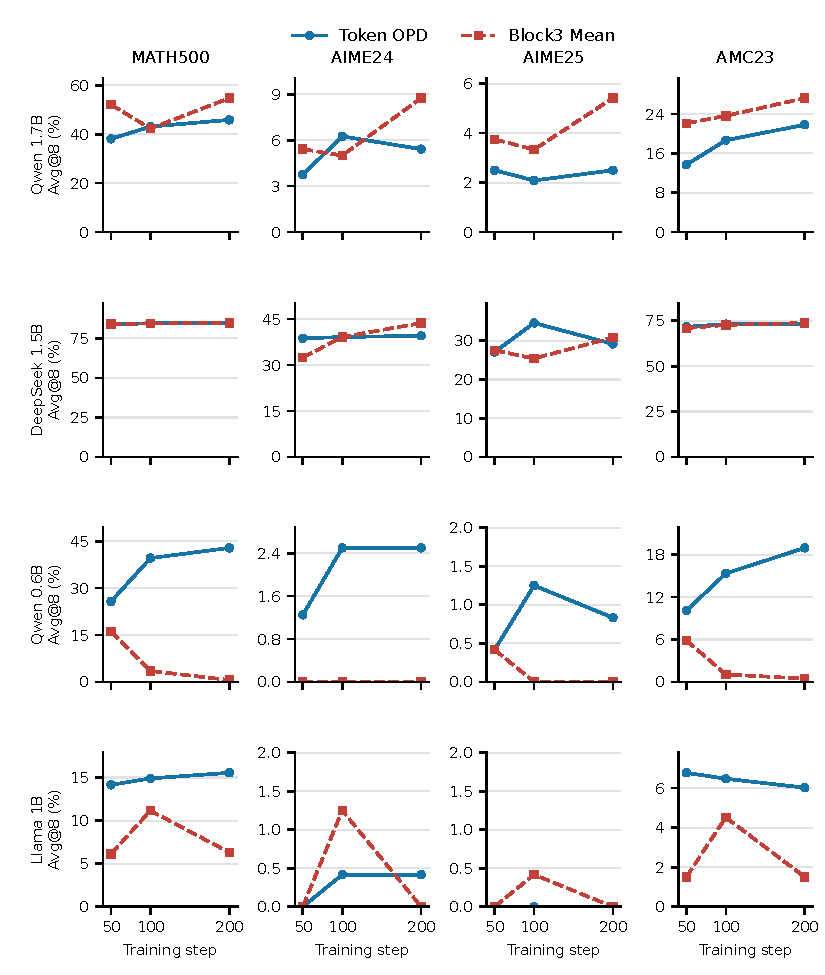
\includegraphics[width=\linewidth]{figures/history_20260921/history_avg_at_8.pdf}
\caption{历史Avg@8权重曲线。Qwen 1.7B采用审计后的external视图，其他行采用保留的historical external视图。每行保持各自协议；均为单训练seed，不是独立多seed复现。各子图纵轴范围不同。连线仅连接三个实测权重，不代表其间存在评测。}
\label{fig:historyavg}
\end{figure}
\begin{figure}[p]
\centering
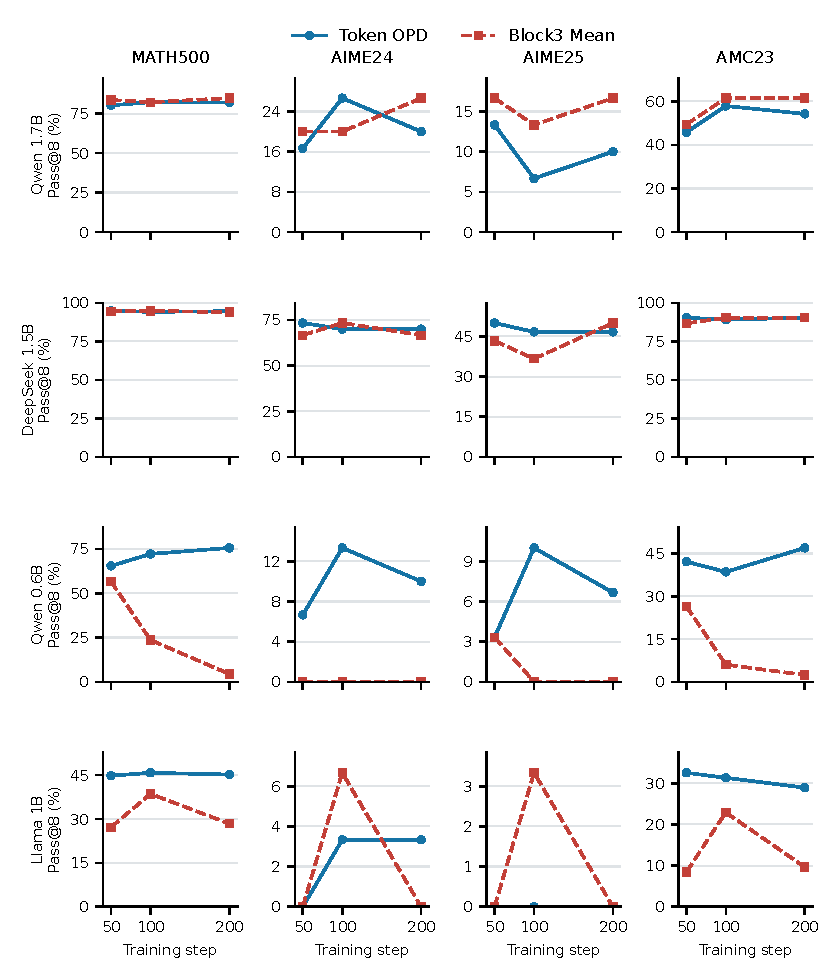
\includegraphics[width=\linewidth]{figures/history_20260921/history_pass_at_8.pdf}
\caption{与图\ref{fig:historyavg}相同权重和协议分层的历史Pass@8。一道题的八个评测响应只要至少一个正确，就贡献一；这与八次正确性指示值的平均不同。图中不隐含独立训练seed上的置信区间。}
\label{fig:historypass}
\end{figure}
\clearpage
\subsection{H01: 早期3400-prompt权重方法与seed7/13 pilot}
\label{history:early_weights50}
训练seed：7, 13；记录训练步数：50。
\paragraph{100-question pilot: mean score / Pass@k, k unrecorded}
{\footnotesize\setlength{\tabcolsep}{3.5pt}
\begin{longtable}{@{}p{1.4in}rrrr@{}}
\toprule
Method & Step & Seed & GSM8K & MATH500 \\
\midrule\endhead
adaptive\_\allowbreak{}exopd & 50 & 7 & 39.00 / 39.00 & 22.00 / 22.00 \\
base & 0 & -- & 43.00 / 43.00 & 22.00 / 22.00 \\
routed\_\allowbreak{}adaptive & 50 & 7 & 40.00 / 40.00 & 26.00 / 26.00 \\
seed13\_\allowbreak{}standard & 50 & 13 & 43.00 / 43.00 & 22.00 / 22.00 \\
seed13\_\allowbreak{}topk\_\allowbreak{}default & 50 & 13 & 38.00 / 38.00 & 27.00 / 27.00 \\
seed7\_\allowbreak{}routed\_\allowbreak{}lam110 & 50 & 7 & 44.00 / 44.00 & 25.00 / 25.00 \\
seed7\_\allowbreak{}topk\_\allowbreak{}strict & 50 & 7 & 41.00 / 41.00 & 20.00 / 20.00 \\
standard & 50 & 7 & 46.00 / 46.00 & 25.00 / 25.00 \\
topk\_\allowbreak{}router & 50 & 7 & 44.00 / 44.00 & 25.00 / 25.00 \\
\bottomrule\end{longtable}
}
\paragraph{Full n=1: original simple grader, accuracy}
{\footnotesize\setlength{\tabcolsep}{3.5pt}
\begin{longtable}{@{}p{1.4in}rrrr@{}}
\toprule
Method & Step & Seed & GSM8K & MATH500 \\
\midrule\endhead
base & 0 & -- & 41.70 & 16.00 \\
routed\_\allowbreak{}lam110 & 50 & 7 & 41.93 & 16.00 \\
standard & 50 & 7 & 41.77 & 16.80 \\
topk\_\allowbreak{}router & 50 & 7 & 41.70 & 16.40 \\
\bottomrule\end{longtable}
}
\paragraph{Full n=1: post-hoc primary grader, accuracy}
{\footnotesize\setlength{\tabcolsep}{3.5pt}
\begin{longtable}{@{}p{1.4in}rrrr@{}}
\toprule
Method & Step & Seed & GSM8K & MATH500 \\
\midrule\endhead
base & 0 & -- & 46.25 & 20.20 \\
routed\_\allowbreak{}lam110 & 50 & 7 & 47.23 & 20.20 \\
standard & 50 & 7 & 46.17 & 20.20 \\
topk\_\allowbreak{}router & 50 & 7 & 46.17 & 19.40 \\
\bottomrule\end{longtable}
}
\subsection{H02: 早期200-step outcome reweight与standard/topk曲线}
\label{history:early_outcome200}
训练seed：7；记录训练步数：200。
\paragraph{Full n=1: original simple grader, accuracy}
{\footnotesize\setlength{\tabcolsep}{3.5pt}
\begin{longtable}{@{}p{1.4in}rrrr@{}}
\toprule
Method & Step & Seed & GSM8K & MATH500 \\
\midrule\endhead
outcome\_\allowbreak{}reweight & 200 & 7 & 33.36 & 12.60 \\
outcome\_\allowbreak{}topk\_\allowbreak{}router & 200 & 7 & 33.21 & 12.20 \\
standard & 100 & 7 & 35.25 & 13.80 \\
standard & 150 & 7 & 33.43 & 12.40 \\
standard & 200 & 7 & 32.15 & 11.80 \\
topk\_\allowbreak{}router & 100 & 7 & 35.25 & 14.20 \\
topk\_\allowbreak{}router & 150 & 7 & 34.87 & 12.00 \\
topk\_\allowbreak{}router & 200 & 7 & 33.89 & 13.20 \\
\bottomrule\end{longtable}
}
\paragraph{Full n=1: post-hoc primary grader, accuracy}
{\footnotesize\setlength{\tabcolsep}{3.5pt}
\begin{longtable}{@{}p{1.4in}rrrr@{}}
\toprule
Method & Step & Seed & GSM8K & MATH500 \\
\midrule\endhead
outcome\_\allowbreak{}reweight & 200 & 7 & 37.83 & 16.60 \\
outcome\_\allowbreak{}topk\_\allowbreak{}router & 200 & 7 & 38.51 & 16.40 \\
standard & 100 & 7 & 39.95 & 16.20 \\
standard & 150 & 7 & 38.06 & 15.80 \\
standard & 200 & 7 & 36.16 & 14.80 \\
topk\_\allowbreak{}router & 100 & 7 & 40.26 & 16.20 \\
topk\_\allowbreak{}router & 150 & 7 & 39.27 & 14.40 \\
topk\_\allowbreak{}router & 200 & 7 & 38.82 & 16.20 \\
\bottomrule\end{longtable}
}
\subsection{H03: 早期100-step reference-anchor对照}
\label{history:early_anchor100}
训练seed：未记录；记录训练步数：100。
\paragraph{Full n=1: original simple grader, accuracy}
{\footnotesize\setlength{\tabcolsep}{3.5pt}
\begin{longtable}{@{}p{1.4in}rrrr@{}}
\toprule
Method & Step & Seed & GSM8K & MATH500 \\
\midrule\endhead
anchored\_\allowbreak{}standard & 100 & -- & 35.41 & 12.40 \\
anchored\_\allowbreak{}topk\_\allowbreak{}router & 100 & -- & 37.15 & 13.40 \\
standard & 100 & -- & 35.48 & 13.40 \\
topk\_\allowbreak{}router & 100 & -- & 34.57 & 14.00 \\
\bottomrule\end{longtable}
}
\paragraph{Full n=1: post-hoc primary grader, accuracy}
{\footnotesize\setlength{\tabcolsep}{3.5pt}
\begin{longtable}{@{}p{1.4in}rrrr@{}}
\toprule
Method & Step & Seed & GSM8K & MATH500 \\
\midrule\endhead
anchored\_\allowbreak{}standard & 100 & -- & 40.03 & 15.20 \\
anchored\_\allowbreak{}topk\_\allowbreak{}router & 100 & -- & 41.93 & 17.80 \\
standard & 100 & -- & 40.71 & 16.80 \\
topk\_\allowbreak{}router & 100 & -- & 39.42 & 17.60 \\
\bottomrule\end{longtable}
}
\subsection{H04: 早期seed7 naive block k1/2/3}
\label{history:early_blocksum50}
训练seed：7；记录训练步数：50。
\paragraph{Full n=1: documented rounded accuracy only}
{\footnotesize\setlength{\tabcolsep}{3.5pt}
\begin{longtable}{@{}p{1.4in}rrrr@{}}
\toprule
Method & Step & Seed & GSM8K & MATH500 \\
\midrule\endhead
block\_\allowbreak{}k2 & 50 & 7 & 45.41 & 19.40 \\
block\_\allowbreak{}k3 & 50 & 7 & 46.85 & 20.20 \\
token\_\allowbreak{}opd & 50 & 7 & 45.94 & 20.00 \\
\bottomrule\end{longtable}
}
\subsection{H05: 早期seed7 Block3 sum/mean/mixed权重}
\label{history:early_blockadv50}
训练seed：7；记录训练步数：50。
\paragraph{Full n=1: documented rounded accuracy only}
{\footnotesize\setlength{\tabcolsep}{3.5pt}
\begin{longtable}{@{}p{1.4in}rrrr@{}}
\toprule
Method & Step & Seed & GSM8K & MATH500 \\
\midrule\endhead
block3\_\allowbreak{}mean & 50 & 7 & 46.93 & 19.80 \\
block3\_\allowbreak{}mixed\_\allowbreak{}lam05 & 50 & 7 & 47.08 & 18.80 \\
block3\_\allowbreak{}sum & 50 & 7 & 46.55 & 19.20 \\
\bottomrule\end{longtable}
}
\subsection{H06: Qwen1.7 Base blocksize sweep k1/3/5/10}
\label{history:qwen17_sweep}
训练seed：21；记录训练步数：200。
\paragraph{Legacy external grader: Avg@8 / Pass@8, evaluation seeds unspecified}
{\footnotesize\setlength{\tabcolsep}{3.5pt}
\begin{longtable}{@{}p{1.4in}rrrrrr@{}}
\toprule
Method & Step & Seed & MATH500 & AIME24 & AIME25 & AMC23 \\
\midrule\endhead
block10\_\allowbreak{}mean & 200 & 21 & 0.00 / 0.00 & 0.00 / 0.00 & 0.00 / 0.00 & 0.00 / 0.00 \\
block3\_\allowbreak{}mean & 200 & 21 & 69.27 / 87.80 & 9.58 / 30.00 & 8.75 / 26.67 & 39.91 / 61.45 \\
block5\_\allowbreak{}mean & 200 & 21 & 67.40 / 87.60 & 9.17 / 20.00 & 7.92 / 23.33 & 34.19 / 61.45 \\
token\_\allowbreak{}opd & 200 & 21 & 69.12 / 88.60 & 13.33 / 26.67 & 6.67 / 16.67 & 36.75 / 62.65 \\
\bottomrule\end{longtable}
}
\subsection{H07: Block10双机独立诊断复跑}
\label{history:block10_collapse}
训练seed：21；记录训练步数：200。
\emph{历史内置AMC23判分存在兼容性问题；零分不等于独立验证的能力测量。}
\paragraph{Built-in grader: Avg@8 / Pass@8 (separate view)}
{\footnotesize\setlength{\tabcolsep}{3.5pt}
\begin{longtable}{@{}p{1.4in}rrrrrr@{}}
\toprule
Method & Step & Seed & MATH500 & AIME24 & AIME25 & AMC23 \\
\midrule\endhead
Block10: A100 host & 50 & 21 & 37.75 / 78.60 & 4.17 / 20.00 & 2.08 / 13.33 & 0.00 / 0.00 \\
Block10: A100 host & 100 & 21 & 0.97 / 7.20 & 0.00 / 0.00 & 0.00 / 0.00 & 0.00 / 0.00 \\
Block10: A100 host & 200 & 21 & 0.00 / 0.00 & 0.00 / 0.00 & 0.00 / 0.00 & 0.00 / 0.00 \\
Block10: A800 host & 50 & 21 & 45.20 / 79.20 & 2.50 / 13.33 & 2.92 / 10.00 & 0.00 / 0.00 \\
Block10: A800 host & 100 & 21 & 2.70 / 16.60 & 0.00 / 0.00 & 0.00 / 0.00 & 0.00 / 0.00 \\
Block10: A800 host & 200 & 21 & 0.00 / 0.00 & 0.00 / 0.00 & 0.00 / 0.00 & 0.00 / 0.00 \\
\bottomrule\end{longtable}
}
\subsection{H08: Qwen1.7 Base 同机Token/Block3严格配对}
\label{history:qwen17_ml2}
训练seed：21；记录训练步数：200。
\emph{历史内置AMC23判分存在兼容性问题；零分不等于独立验证的能力测量。}
\paragraph{Built-in grader: Avg@8 / Pass@8 (separate view)}
{\footnotesize\setlength{\tabcolsep}{3.5pt}
\begin{longtable}{@{}p{1.4in}rrrrrr@{}}
\toprule
Method & Step & Seed & MATH500 & AIME24 & AIME25 & AMC23 \\
\midrule\endhead
block3\_\allowbreak{}mean & 50 & 21 & 50.25 / 81.00 & 5.42 / 20.00 & 3.75 / 16.67 & 0.00 / 0.00 \\
block3\_\allowbreak{}mean & 100 & 21 & 40.80 / 80.40 & 5.00 / 20.00 & 3.33 / 13.33 & 0.00 / 0.00 \\
block3\_\allowbreak{}mean & 200 & 21 & 52.83 / 82.20 & 8.75 / 26.67 & 5.42 / 16.67 & 0.00 / 0.00 \\
token\_\allowbreak{}opd & 50 & 21 & 37.05 / 78.00 & 3.75 / 16.67 & 2.50 / 13.33 & 0.00 / 0.00 \\
token\_\allowbreak{}opd & 100 & 21 & 41.80 / 80.20 & 6.25 / 26.67 & 2.08 / 6.67 & 0.00 / 0.00 \\
token\_\allowbreak{}opd & 200 & 21 & 44.45 / 80.00 & 5.42 / 20.00 & 2.50 / 10.00 & 0.00 / 0.00 \\
\bottomrule\end{longtable}
}
\paragraph{Audited historical external grader: Avg@8 / Pass@8}
{\footnotesize\setlength{\tabcolsep}{3.5pt}
\begin{longtable}{@{}p{1.4in}rrrrrr@{}}
\toprule
Method & Step & Seed & MATH500 & AIME24 & AIME25 & AMC23 \\
\midrule\endhead
block3\_\allowbreak{}mean & 50 & 21 & 52.10 / 83.60 & 5.42 / 20.00 & 3.75 / 16.67 & 22.14 / 49.40 \\
block3\_\allowbreak{}mean & 100 & 21 & 42.27 / 82.20 & 5.00 / 20.00 & 3.33 / 13.33 & 23.64 / 61.45 \\
block3\_\allowbreak{}mean & 200 & 21 & 54.75 / 84.80 & 8.75 / 26.67 & 5.42 / 16.67 & 27.26 / 61.45 \\
token\_\allowbreak{}opd & 50 & 21 & 38.07 / 80.20 & 3.75 / 16.67 & 2.50 / 13.33 & 13.70 / 45.78 \\
token\_\allowbreak{}opd & 100 & 21 & 43.10 / 82.20 & 6.25 / 26.67 & 2.08 / 6.67 & 18.67 / 57.83 \\
token\_\allowbreak{}opd & 200 & 21 & 45.85 / 82.00 & 5.42 / 20.00 & 2.50 / 10.00 & 21.84 / 54.22 \\
\bottomrule\end{longtable}
}
\subsection{H09: Qwen1.7历史六权重新生成评测}
\label{history:qwen17_reeval}
训练seed：21；记录训练步数：--。
\paragraph{Historical external grader: Avg@8 / Pass@8}
{\footnotesize\setlength{\tabcolsep}{3.5pt}
\begin{longtable}{@{}p{1.4in}rrrrrr@{}}
\toprule
Method & Step & Seed & MATH500 & AIME24 & AIME25 & AMC23 \\
\midrule\endhead
block3\_\allowbreak{}mean & 50 & 21 & 52.05 / 84.60 & 5.00 / 16.67 & 3.33 / 16.67 & 23.80 / 51.81 \\
block3\_\allowbreak{}mean & 100 & 21 & 42.65 / 83.00 & 5.00 / 20.00 & 2.50 / 13.33 & 23.49 / 56.63 \\
block3\_\allowbreak{}mean & 200 & 21 & 54.15 / 84.00 & 7.08 / 26.67 & 5.83 / 16.67 & 29.22 / 65.06 \\
token\_\allowbreak{}opd & 50 & 21 & 38.30 / 81.80 & 2.50 / 16.67 & 3.75 / 16.67 & 14.61 / 51.81 \\
token\_\allowbreak{}opd & 100 & 21 & 43.35 / 83.00 & 6.25 / 20.00 & 2.08 / 6.67 & 18.52 / 55.42 \\
token\_\allowbreak{}opd & 200 & 21 & 45.92 / 83.00 & 6.67 / 16.67 & 3.75 / 10.00 & 23.34 / 60.24 \\
\bottomrule\end{longtable}
}
\subsection{H10: DeepSeek-R1-Distill/JustRL配对}
\label{history:deepseek_justrl}
训练seed：21；记录训练步数：200。
\paragraph{Historical external grader: Avg@8 / Pass@8}
{\footnotesize\setlength{\tabcolsep}{3.5pt}
\begin{longtable}{@{}p{1.4in}rrrrrr@{}}
\toprule
Method & Step & Seed & MATH500 & AIME24 & AIME25 & AMC23 \\
\midrule\endhead
block3\_\allowbreak{}mean & 50 & 21 & 84.15 / 94.60 & 32.50 / 66.67 & 27.50 / 43.33 & 70.93 / 86.75 \\
block3\_\allowbreak{}mean & 100 & 21 & 84.45 / 94.80 & 39.17 / 73.33 & 25.42 / 36.67 & 72.74 / 90.36 \\
block3\_\allowbreak{}mean & 200 & 21 & 84.75 / 94.00 & 43.75 / 66.67 & 30.83 / 50.00 & 73.80 / 90.36 \\
token\_\allowbreak{}opd & 50 & 21 & 83.78 / 94.80 & 38.75 / 73.33 & 27.08 / 50.00 & 71.69 / 90.36 \\
token\_\allowbreak{}opd & 100 & 21 & 84.62 / 94.20 & 39.17 / 70.00 & 34.58 / 46.67 & 73.19 / 89.16 \\
token\_\allowbreak{}opd & 200 & 21 & 84.70 / 94.60 & 39.58 / 70.00 & 29.17 / 46.67 & 73.34 / 90.36 \\
\bottomrule\end{longtable}
}
\emph{历史内置AMC23判分存在兼容性问题；零分不等于独立验证的能力测量。}
\paragraph{Built-in grader: Avg@8 / Pass@8 (separate view)}
{\footnotesize\setlength{\tabcolsep}{3.5pt}
\begin{longtable}{@{}p{1.4in}rrrrrr@{}}
\toprule
Method & Step & Seed & MATH500 & AIME24 & AIME25 & AMC23 \\
\midrule\endhead
block3\_\allowbreak{}mean & 50 & 21 & 81.80 / 91.60 & 32.50 / 66.67 & 27.50 / 43.33 & 0.00 / 0.00 \\
block3\_\allowbreak{}mean & 100 & 21 & 82.23 / 91.80 & 39.17 / 73.33 & 25.42 / 36.67 & 0.00 / 0.00 \\
block3\_\allowbreak{}mean & 200 & 21 & 82.25 / 90.80 & 43.75 / 66.67 & 30.83 / 50.00 & 0.00 / 0.00 \\
token\_\allowbreak{}opd & 50 & 21 & 81.47 / 91.60 & 38.75 / 73.33 & 27.08 / 50.00 & 0.00 / 0.00 \\
token\_\allowbreak{}opd & 100 & 21 & 82.12 / 91.00 & 39.17 / 70.00 & 34.58 / 46.67 & 0.00 / 0.00 \\
token\_\allowbreak{}opd & 200 & 21 & 82.25 / 91.60 & 39.58 / 70.00 & 29.17 / 46.67 & 0.00 / 0.00 \\
\bottomrule\end{longtable}
}
\subsection{H11: Qwen1.7 random3/sliding3}
\label{history:window_random_sliding}
训练seed：21；记录训练步数：200。
\paragraph{Historical external grader: Avg@8 / Pass@8}
{\footnotesize\setlength{\tabcolsep}{3.5pt}
\begin{longtable}{@{}p{1.4in}rrrrrr@{}}
\toprule
Method & Step & Seed & MATH500 & AIME24 & AIME25 & AMC23 \\
\midrule\endhead
random3 & 50 & 21 & 45.23 / 81.60 & 5.00 / 20.00 & 2.92 / 10.00 & 18.22 / 48.19 \\
random3 & 100 & 21 & 36.70 / 82.40 & 2.08 / 13.33 & 1.67 / 10.00 & 14.91 / 48.19 \\
random3 & 200 & 21 & 21.18 / 73.60 & 3.33 / 16.67 & 0.00 / 0.00 & 12.20 / 46.99 \\
sliding3 & 50 & 21 & 41.33 / 81.80 & 3.75 / 23.33 & 1.67 / 10.00 & 15.66 / 48.19 \\
sliding3 & 100 & 21 & 52.08 / 85.20 & 4.58 / 20.00 & 2.92 / 10.00 & 24.85 / 57.83 \\
sliding3 & 200 & 21 & 34.75 / 81.00 & 5.00 / 20.00 & 2.08 / 10.00 & 15.81 / 48.19 \\
\bottomrule\end{longtable}
}
\emph{历史内置AMC23判分存在兼容性问题；零分不等于独立验证的能力测量。}
\paragraph{Built-in grader: Avg@8 / Pass@8 (separate view)}
{\footnotesize\setlength{\tabcolsep}{3.5pt}
\begin{longtable}{@{}p{1.4in}rrrrrr@{}}
\toprule
Method & Step & Seed & MATH500 & AIME24 & AIME25 & AMC23 \\
\midrule\endhead
random3 & 50 & 21 & 43.43 / 79.00 & 5.00 / 20.00 & 2.92 / 10.00 & 0.00 / 0.00 \\
random3 & 100 & 21 & 35.27 / 79.60 & 2.08 / 13.33 & 1.67 / 10.00 & 0.00 / 0.00 \\
random3 & 200 & 21 & 20.50 / 71.60 & 3.33 / 16.67 & 0.00 / 0.00 & 0.00 / 0.00 \\
sliding3 & 50 & 21 & 40.02 / 79.20 & 3.75 / 23.33 & 1.67 / 10.00 & 0.00 / 0.00 \\
sliding3 & 100 & 21 & 50.42 / 82.80 & 4.58 / 20.00 & 2.92 / 10.00 & 0.00 / 0.00 \\
sliding3 & 200 & 21 & 33.70 / 78.00 & 5.00 / 20.00 & 2.08 / 10.00 & 0.00 / 0.00 \\
\bottomrule\end{longtable}
}
\subsection{H12: Qwen0.6 Base旧thinking-unspecified提示}
\label{history:qwen06_old_prompt}
训练seed：21；记录训练步数：200。
\paragraph{Incomplete planned evaluation: no full benchmark claim}
{\footnotesize\setlength{\tabcolsep}{3.5pt}
\begin{longtable}{@{}p{1.4in}rrrrrr@{}}
\toprule
Method & Step & Seed & MATH500 & AIME24 & AIME25 & AMC23 \\
\midrule\endhead
token\_\allowbreak{}opd & 50 & 21 & -- & -- & -- & -- \\
token\_\allowbreak{}opd & 100 & 21 & -- & -- & -- & -- \\
token\_\allowbreak{}opd & 200 & 21 & -- & -- & -- & -- \\
\bottomrule\end{longtable}
}
\subsection{H13: Qwen0.6 Base显式非thinking配对}
\label{history:qwen06_nonthinking}
训练seed：21；记录训练步数：200。
\paragraph{Historical external grader: Avg@8 / Pass@8}
{\footnotesize\setlength{\tabcolsep}{3.5pt}
\begin{longtable}{@{}p{1.4in}rrrrrr@{}}
\toprule
Method & Step & Seed & MATH500 & AIME24 & AIME25 & AMC23 \\
\midrule\endhead
block3\_\allowbreak{}mean & 50 & 21 & 16.20 / 56.60 & 0.00 / 0.00 & 0.42 / 3.33 & 5.87 / 26.51 \\
block3\_\allowbreak{}mean & 100 & 21 & 3.48 / 23.60 & 0.00 / 0.00 & 0.00 / 0.00 & 1.05 / 6.02 \\
block3\_\allowbreak{}mean & 200 & 21 & 0.57 / 4.40 & 0.00 / 0.00 & 0.00 / 0.00 & 0.45 / 2.41 \\
student\_\allowbreak{}base & 0 & -- & 10.45 / 45.20 & 0.42 / 3.33 & 0.00 / 0.00 & 3.46 / 24.10 \\
teacher & 0 & -- & 83.43 / 93.40 & 23.33 / 43.33 & 18.75 / 26.67 & 57.68 / 77.11 \\
token\_\allowbreak{}opd & 50 & 21 & 25.70 / 65.40 & 1.25 / 6.67 & 0.42 / 3.33 & 10.09 / 42.17 \\
token\_\allowbreak{}opd & 100 & 21 & 39.60 / 72.20 & 2.50 / 13.33 & 1.25 / 10.00 & 15.36 / 38.55 \\
token\_\allowbreak{}opd & 200 & 21 & 42.88 / 75.60 & 2.50 / 10.00 & 0.83 / 6.67 & 18.98 / 46.99 \\
\bottomrule\end{longtable}
}
\subsection{H14: Llama3.2原生非thinking提示尝试}
\label{history:llama_native_stopped}
训练seed：21；记录训练步数：146。
\paragraph{Historical external grader: Avg@8 / Pass@8}
{\footnotesize\setlength{\tabcolsep}{3.5pt}
\begin{longtable}{@{}p{1.4in}rrrrrr@{}}
\toprule
Method & Step & Seed & MATH500 & AIME24 & AIME25 & AMC23 \\
\midrule\endhead
student\_\allowbreak{}base & 0 & -- & 13.80 / 45.20 & 0.42 / 3.33 & 0.00 / 0.00 & 4.07 / 21.69 \\
token\_\allowbreak{}opd & 50 & 21 & -- & -- & -- & -- \\
token\_\allowbreak{}opd & 100 & 21 & -- & -- & -- & -- \\
token\_\allowbreak{}opd & 200 & 21 & -- & -- & -- & -- \\
\bottomrule\end{longtable}
}
\subsection{H15: Llama3.2 historical17训推差异配对}
\label{history:llama_historical}
训练seed：21；记录训练步数：200。
\paragraph{Historical external grader: Avg@8 / Pass@8}
{\footnotesize\setlength{\tabcolsep}{3.5pt}
\begin{longtable}{@{}p{1.4in}rrrrrr@{}}
\toprule
Method & Step & Seed & MATH500 & AIME24 & AIME25 & AMC23 \\
\midrule\endhead
block3\_\allowbreak{}mean & 50 & 21 & 6.12 / 27.20 & 0.00 / 0.00 & 0.00 / 0.00 & 1.51 / 8.43 \\
block3\_\allowbreak{}mean & 100 & 21 & 11.15 / 38.60 & 1.25 / 6.67 & 0.42 / 3.33 & 4.52 / 22.89 \\
block3\_\allowbreak{}mean & 200 & 21 & 6.30 / 28.40 & 0.00 / 0.00 & 0.00 / 0.00 & 1.51 / 9.64 \\
student\_\allowbreak{}base & 0 & -- & 14.00 / 46.40 & 0.42 / 3.33 & 0.00 / 0.00 & 5.27 / 28.92 \\
token\_\allowbreak{}opd & 50 & 21 & 14.15 / 44.80 & 0.00 / 0.00 & 0.00 / 0.00 & 6.78 / 32.53 \\
token\_\allowbreak{}opd & 100 & 21 & 14.90 / 45.80 & 0.42 / 3.33 & 0.00 / 0.00 & 6.48 / 31.33 \\
token\_\allowbreak{}opd & 200 & 21 & 15.55 / 45.20 & 0.42 / 3.33 & 0.00 / 0.00 & 6.02 / 28.92 \\
\bottomrule\end{longtable}
}
\subsection{H16: Qwen4旧ChatML Block3-first失败/中止}
\label{history:qwen4_chatml_stopped}
训练seed：21；记录训练步数：4。
此尝试无已完成benchmark结果记录。
\subsection{H17: Qwen4新completion Block3与新Token}
\label{history:qwen4_completion}
训练seed：21；记录训练步数：200。
该师生对的最终结果见附录\ref{app:current}。


\section{有限规模的提示诊断}
\label{app:probes}
这些是在选定训练题上的推理 probe，不是额外的保留测试集 benchmark 成绩。Qwen3-4B 和 Llama 提示研究每个条件使用固定 16 题、每题两个独立 seed（21、22）响应。Qwen 0.6/1.7 的主要诊断与前 16 题消融保留各自样本数，不把重叠题目相加当作独立观测。表中均为整数计数：长度终止、周期性尾部、缺失字面 boxed 标记和正确判分的响应数；横线表示未记录。周期尾部检测要求至少 256 个尾部 token，在最后 2,048 个 token 内存在不超过 128 的偏移，使 token 一致率至少为 99\%；它是一个检测器，不是完整的语义重复指标。

历史训练 user 消息为：
\begin{quote}\small
\texttt{Math problem: [question]}\\
\texttt{Please carefully reason through the math problem step by step and derive the correct answer. You must conduct reasoning inside <think> and </think> and give the final answer within}\ \verb|\boxed{}.|\
\end{quote}
模型原生模板在这段内容外添加聊天边界及 assistant 生成前缀。“No think”只删除 \texttt{conduct reasoning inside <think> and </think> and} 这一短语，并不等于绕过 chat template。历史评测使用题目与 \texttt{Please reason step by step, and put your final answer within} \verb|\boxed{}.|，同时显式关闭 thinking。因此，请求推理标签与关闭原生 thinking 模式是不同的控制。

Qwen3-4B 的“plain”是裸题目、两个换行及 \texttt{Solution:}；“candidate”是第~\ref{sec:protocol} 节最终配对的 completion 协议。Llama 的“completion”保留移除 think 要求后的历史指令与一个原生 BOS，去掉聊天角色边界并追加 \texttt{Solution:}，并不等于 Qwen 的 plain 条件。“eval”使用 Llama 原生的非 thinking 评测模板。在这组 probe 中，去 chat 使 Llama 学生的长度终止从 1/32 升到 4/32；而 Qwen3-4B 从 historical 改为 candidate 后，由 18/32 降至 1/32。这支持按模型进行验证，而不是对指令模型普遍移除聊天格式。
\paragraph{Llama prompt}
{\small\setlength{\tabcolsep}{4pt}
\begin{longtable}{@{}llrrrrr@{}}
\toprule
Model & Condition & $n$ & Length & Periodic & No box & Correct \\
\midrule\endhead
student & historical & 32 & 1 & 1 & 10 & 0 \\
student & no\_\allowbreak{}think & 32 & 1 & 0 & 16 & 1 \\
student & completion & 32 & 4 & 1 & 3 & 1 \\
student & eval & 32 & 1 & 1 & 11 & 0 \\
teacher & historical & 32 & 2 & 1 & 6 & 3 \\
teacher & no\_\allowbreak{}think & 32 & 4 & 2 & 9 & 2 \\
teacher & completion & 32 & 4 & 2 & 2 & 1 \\
teacher & eval & 32 & 0 & 0 & 6 & 2 \\
\bottomrule\end{longtable}
}
\paragraph{Qwen3-4B prompt}
{\small\setlength{\tabcolsep}{4pt}
\begin{longtable}{@{}llrrrrr@{}}
\toprule
Model & Condition & $n$ & Length & Periodic & No box & Correct \\
\midrule\endhead
student & historical & 32 & 18 & 17 & 21 & 1 \\
student & plain & 32 & 0 & 0 & 9 & 2 \\
student & candidate & 32 & 1 & 1 & 0 & 4 \\
teacher & historical & 32 & 2 & 0 & 2 & 6 \\
teacher & plain & 32 & 0 & 0 & 0 & 5 \\
teacher & candidate & 32 & 3 & 2 & 2 & 8 \\
\bottomrule\end{longtable}
}
\paragraph{Qwen 0.6/1.7 primary32}
{\small\setlength{\tabcolsep}{4pt}
\begin{longtable}{@{}llrrrrr@{}}
\toprule
Model & Condition & $n$ & Length & Periodic & No box & Correct \\
\midrule\endhead
q06\_\allowbreak{}base & -- & 32 & 12 & 10 & -- & 0 \\
q06\_\allowbreak{}step50 & -- & 32 & 10 & 4 & -- & 1 \\
q17\_\allowbreak{}base & -- & 32 & 16 & 10 & -- & 1 \\
q17\_\allowbreak{}step50 & -- & 32 & 4 & 0 & -- & 4 \\
\bottomrule\end{longtable}
}
\paragraph{Qwen 0.6/1.7 prompt\_\allowbreak{}ablation\_\allowbreak{}first16}
{\small\setlength{\tabcolsep}{4pt}
\begin{longtable}{@{}llrrrrr@{}}
\toprule
Model & Condition & $n$ & Length & Periodic & No box & Correct \\
\midrule\endhead
q06\_\allowbreak{}base\_\allowbreak{}no\_\allowbreak{}think & -- & 16 & 5 & 4 & -- & 1 \\
q06\_\allowbreak{}base\_\allowbreak{}plain & -- & 16 & 1 & 1 & -- & 1 \\
q06\_\allowbreak{}base\_\allowbreak{}training & -- & 16 & 6 & 6 & -- & 0 \\
q17\_\allowbreak{}base\_\allowbreak{}no\_\allowbreak{}think & -- & 16 & 1 & 1 & -- & 1 \\
q17\_\allowbreak{}base\_\allowbreak{}plain & -- & 16 & 0 & 0 & -- & 0 \\
q17\_\allowbreak{}base\_\allowbreak{}training & -- & 16 & 6 & 4 & -- & 1 \\
\bottomrule\end{longtable}
}


\section{4B Base的全部Checkpoint结果}
\label{app:current}
当前师生对使用附录~\ref{app:config} 中的配对 completion 协议。分数以百分数而非小数表示；差异为同一权重步、同一 benchmark 上的 Block3 减去 Token。缺失 boxed 标记比例和引擎长度终止比例使用每题全部八条响应；Avg@8 与 Pass@8 定义见式~\ref{eq:metrics}。不同权重的比较描述每种方法的一条训练轨迹，不能解释为独立重复实验。
% Generated; do not edit. Requires booktabs; Chinese requires CJK support.
\begin{table*}[t]
\centering
\small
\caption{Qwen3-4B completion，seed21，COMPLETE。分数单位为百分比，NA表示缺失。}
\begin{tabular}{lllrrrr}
\toprule
基准 & 方法 & 步数 & Avg@8 & Pass@8 & 缺box & 截断 \\
\midrule
MATH500 & Block3 Mean & 200 & 75.40 & 90.60 & 0.90 & 0.90 \\
MATH500 & Block3 Mean & 150 & 78.03 & 91.20 & 0.83 & 0.83 \\
MATH500 & Block3 Mean & 100 & 75.52 & 90.80 & 1.25 & 1.18 \\
MATH500 & Block3 Mean & 50 & 78.53 & 91.80 & 0.85 & 0.75 \\
MATH500 & Token OPD & 200 & 75.92 & 91.00 & 0.85 & 0.80 \\
MATH500 & Token OPD & 150 & 76.17 & 91.40 & 0.95 & 0.97 \\
MATH500 & Token OPD & 100 & 76.92 & 90.40 & 1.07 & 0.95 \\
MATH500 & Token OPD & 50 & 78.65 & 92.20 & 0.85 & 0.80 \\
\midrule
AIME24 & Block3 Mean & 200 & 13.33 & 33.33 & 12.08 & 11.25 \\
AIME24 & Block3 Mean & 150 & 15.42 & 33.33 & 9.58 & 8.75 \\
AIME24 & Block3 Mean & 100 & 15.00 & 30.00 & 13.75 & 12.08 \\
AIME24 & Block3 Mean & 50 & 14.17 & 30.00 & 7.08 & 6.25 \\
AIME24 & Token OPD & 200 & 16.25 & 30.00 & 7.92 & 6.67 \\
AIME24 & Token OPD & 150 & 12.50 & 26.67 & 10.42 & 8.33 \\
AIME24 & Token OPD & 100 & 12.92 & 26.67 & 12.08 & 9.17 \\
AIME24 & Token OPD & 50 & 17.92 & 36.67 & 10.42 & 8.75 \\
\midrule
AIME25 & Block3 Mean & 200 & 13.75 & 30.00 & 4.17 & 3.33 \\
AIME25 & Block3 Mean & 150 & 11.67 & 26.67 & 5.42 & 5.42 \\
AIME25 & Block3 Mean & 100 & 12.08 & 33.33 & 7.50 & 6.25 \\
AIME25 & Block3 Mean & 50 & 11.67 & 23.33 & 7.50 & 5.42 \\
AIME25 & Token OPD & 200 & 13.33 & 30.00 & 3.75 & 3.33 \\
AIME25 & Token OPD & 150 & 15.83 & 40.00 & 5.42 & 6.25 \\
AIME25 & Token OPD & 100 & 10.83 & 23.33 & 5.83 & 5.42 \\
AIME25 & Token OPD & 50 & 12.92 & 23.33 & 7.08 & 4.17 \\
\midrule
AMC23 & Block3 Mean & 200 & 46.23 & 74.70 & 4.52 & 4.07 \\
AMC23 & Block3 Mean & 150 & 49.70 & 77.11 & 3.46 & 3.01 \\
AMC23 & Block3 Mean & 100 & 47.29 & 74.70 & 3.92 & 3.01 \\
AMC23 & Block3 Mean & 50 & 50.30 & 74.70 & 4.37 & 3.31 \\
AMC23 & Token OPD & 200 & 49.25 & 77.11 & 3.61 & 3.01 \\
AMC23 & Token OPD & 150 & 49.40 & 77.11 & 2.56 & 2.86 \\
AMC23 & Token OPD & 100 & 49.25 & 78.31 & 2.56 & 2.56 \\
AMC23 & Token OPD & 50 & 48.49 & 78.31 & 3.16 & 3.01 \\
\bottomrule
\end{tabular}
\par\smallskip\footnotesize 缺box仅指无字面标记 \texttt{\textbackslash boxed}；截断指引擎 length 终止。
\end{table*}


配对题目 bootstrap 区间在每个 benchmark 内独立计算，两组共同重采样相同题目身份，并条件化于每题已保留的八条响应及已训练权重。它不重采样训练 seed，不估计教师不确定性，也不提供跨多个权重或 benchmark 的同时覆盖保证。百分位方法使用 10,000 次重采样，seed 为 20260921。置信区间跨过零不证明两种方法等效。

\begin{figure}[t]
\centering

\includegraphics[width=\linewidth]{\qwenfigures/qwen4_pass.pdf}
\caption{当前配对实验四个权重的Pass@8。各任务纵轴范围独立，同一子图内两种方法共享范围。每个点使用全部题目、每题八条响应，并非选择部分输出。}
\end{figure}

\paragraph{事后重叠敏感性分析。}
剔除附录\ref{app:config}中的四道训练池字符串重叠题后，MATH500剩余496题。Step200的Avg@8差值为$-0.58$个百分点（$[-1.66,0.50]$），完整benchmark为$-0.52$。Step50/100/150的差值符号也未改变。这不能排除语义重叠或上游模型训练污染，不能估计污染的因果作用，也不构成新的留出benchmark。完整500题结果仍为主要报告。
% Generated post-hoc sensitivity only; requires booktabs and CJK for Chinese.
\begin{table*}[t]
\centering
\scriptsize
\setlength{\tabcolsep}{4pt}
\caption{事后重叠敏感性分析：MATH500的496题子集 (COMPLETE)。}
\label{tab:qwen4overlapsensitivity}
\begin{tabular}{lrrrrrr}
\toprule
 & \multicolumn{3}{c}{Avg@8} & \multicolumn{3}{c}{Pass@8} \\
\cmidrule(lr){2-4}\cmidrule(lr){5-7}
步数 & Block3 & Token & $\Delta$ & Block3 & Token & $\Delta$ \\
\midrule
200 & 75.73 & 76.31 & -0.58 [-1.66, 0.50] & 90.73 & 91.33 & -0.60 [-2.62, 1.21] \\
150 & 78.40 & 76.56 & +1.84 & 91.53 & 91.53 & +0.00 \\
100 & 75.83 & 77.27 & -1.44 & 90.93 & 90.52 & +0.40 \\
50 & 78.93 & 79.08 & -0.15 & 91.94 & 92.34 & -0.40 \\
\bottomrule
\end{tabular}
\par\smallskip\footnotesize 剔除审计中空白折叠加casefold匹配的4题，包含2题精确匹配。仅为事后敏感性分析，不是新基准或主结果；官方全500题分数不变。分数为百分比；$\Delta$为Block3减Token的百分点差；NA表示缺少配对题目分数。 仅Step200方括号为496题内配对问题bootstrap的逐点95\%区间；条件于一对训练运行，非多训练种子CI。
\end{table*}


\begin{figure}[htbp]
\centering

\includegraphics[width=\linewidth]{\qwendiagnostics/qwen4_training.pdf}
\caption{4B逐步训练诊断。熵是学生前缀上的全词表、更新前统计，梯度范数是裁剪前诊断。底图衡量训练响应触及上限，不是评测引擎停止原因；曲线不确立性能差异的成因。}
\label{fig:qwen4training}
\end{figure}
\FloatBarrier

\section{官方Qwen3-8B到1.7B指令版对照}
\label{app:instruct}
\paragraph{独立的官方指令模型分层。}
教师为\texttt{Qwen/Qwen3-8B}，ModelScope revision为
\texttt{26028140be3ee69b82b1d1450179ab71bb1121b9}；学生为
\texttt{Qwen/Qwen3-1.7B}，revision为\texttt{4855588ea1a12789f2e965e5f52a9e4a24c94b2a}。
二者都是官方后训练模型，仓库名称不包含Instruct字样，但均不是Base权重。
本组与附录\ref{app:history}中历史1.7B学生/公开GRPO教师的实验分开报告。
Token与Block3分别从同一原始学生独立初始化，采用同一保留DAPO训练池、seed21、
200步、每步4题每题8条、学习率$2\times10^{-6}$及四个保存权重。
优化器、裁剪和micro-batch沿用附录\ref{app:config}中的共同配置。
历史Block3目标未改动，因而仍不是仅修改advantage的消融。
两组各6,400条轨迹的输入与请求seed已逐项配对审计；复用同一数据不是独立数据集复现，
也不会消除训练池原有的重叠风险。

\paragraph{原生非thinking提示。}
与4B Base的completion分层不同，本组保留Qwen原生chat template。
单条user消息由去除首尾空白的题面、两个换行，以及
\texttt{Please solve the problem step by step and put the final answer in}
\verb|\boxed{}.|构成，不追加\texttt{Solution:}。
训练与评测均显式设置\texttt{enable\_thinking=False}及
\texttt{add\_generation\_prompt=True}。
模板生成的空闭合\texttt{<think>...</think>}控制前缀属于输入，不是模型生成的推理。
EOS为151645，停止集合为$\{151645,151643\}$；有效响应长度不包含padding尾部。
真实collector、教师与评测输入token ID均核验一致；普通文字逐步解题仍然允许。

\paragraph{评测与恢复来源。}
原始学生、两种算法的Step50/100/150/200均完整评测四项benchmark，
使用同一固定历史grader、seed21至28、temperature1.0、top-$p=0.9$及16,384-token上限。
共9个模型视图、46,296条评测响应。归档标签\texttt{student\_base}指训练前的指令版学生，
不是Base模型。最初的Token启动在Ray初始化时失败，尚无正式更新；成功重试保留冻结训练实现，
并从原始学生独立初始化。已经验收的Block3与原始学生评测直接复用，没有重生成或算成额外实验。
所有训练和评测原始轨迹均保留。

\paragraph{完整权重而非挑选最佳。}
表\ref{tab:qwen17avgall}和\ref{tab:qwen17passall}保留全部保存权重。
Step50的四项Avg@8中三项更有利于Token，Step150的AIME24也更有利于Token。
本组MATH500最高Avg@8来自Token Step100，而不是Block3 Step200。
最终端点两方法的四项Avg@8均高于原始学生，但MATH500 Pass@8均更低：
89.60\%和89.80\%，原始学生为91.20\%。这不支持八次尝试覆盖率全面提升。
正文端点表采用10,000次配对题目重采样，bootstrap seed为20260923。
区间条件固定为这一个训练seed及已有响应，不是训练seed区间，也未校正多个权重/benchmark比较。
Step200的全部Avg@8和Pass@8区间均包含零；这也不意味着证明了等效。

\begin{table}[htbp]
\centering\small
\caption{官方8B到1.7B指令版：完整Avg@8（\%），包括原始学生；各benchmark独立计分。}
\label{tab:qwen17avgall}
\begin{tabular}{lrrrr}
\toprule
Model / Step & MATH500 & AIME24 & AIME25 & AMC23 \\
\midrule
原始学生 & 71.45 & 10.00 & 10.42 & 40.51 \\
Token 50 & 72.47 & 13.33 & 8.75 & 45.48 \\
Block3 50 & 71.50 & 12.50 & 9.58 & 43.67 \\
Token 100 & 72.92 & 15.00 & 12.08 & 43.98 \\
Block3 100 & 72.55 & 16.25 & 13.33 & 44.43 \\
Token 150 & 72.47 & 15.42 & 10.00 & 43.83 \\
Block3 150 & 72.62 & 13.33 & 12.08 & 46.84 \\
Token 200 & 72.12 & 14.17 & 12.08 & 43.07 \\
Block3 200 & 72.22 & 16.67 & 12.92 & 43.37 \\
\bottomrule
\end{tabular}

\end{table}
\begin{table}[htbp]
\centering\small
\caption{相同模型视图的Pass@8（\%）。每题八次尝试不是八次独立训练。}
\label{tab:qwen17passall}
\begin{tabular}{lrrrr}
\toprule
Model / Step & MATH500 & AIME24 & AIME25 & AMC23 \\
\midrule
原始学生 & 91.20 & 26.67 & 23.33 & 69.88 \\
Token 50 & 90.60 & 33.33 & 26.67 & 73.49 \\
Block3 50 & 89.00 & 26.67 & 16.67 & 73.49 \\
Token 100 & 89.00 & 30.00 & 30.00 & 69.88 \\
Block3 100 & 91.00 & 36.67 & 33.33 & 68.67 \\
Token 150 & 90.60 & 30.00 & 26.67 & 71.08 \\
Block3 150 & 91.60 & 30.00 & 36.67 & 74.70 \\
Token 200 & 89.60 & 43.33 & 30.00 & 75.90 \\
Block3 200 & 89.80 & 36.67 & 30.00 & 74.70 \\
\bottomrule
\end{tabular}

\end{table}
\FloatBarrier

\paragraph{行为指标并非全面改善。}
训练中Token有94/6,400条引擎长度终止（1.47\%），Block3为77/6,400（1.20\%），
两组均未生成thinking标签。最大记录裁剪前梯度范数分别为5.13与6.90。
这些有限诊断数值不证明更好的数学推理或更低的梯度方差。
全部9次评测的生成thinking标签计数均为零，但表\ref{tab:qwen17behavior}显示，
缺失boxed标记和长度终止的差异依赖benchmark：AIME24上Block3两者都更多，
AIME25和AMC23上则更少。历史格式指标只检查缺失字面boxed标记，
不是完整语法、答案提取或数学正确性的审计。

\begin{table}[htbp]
\centering\scriptsize
\caption{官方指令版Step200行为比例（\%）。缺失box标记与引擎长度终止分别统计，分母均为全部响应。}
\label{tab:qwen17behavior}
\begin{tabular}{lrrrr}
\toprule
Benchmark & Token missing box & Block3 missing box & Token length & Block3 length \\
\midrule
MATH500 & 0.125 & 0.150 & 0.175 & 0.150 \\
AIME24 & 1.667 & 2.083 & 1.667 & 2.500 \\
AIME25 & 0.417 & 0.000 & 0.417 & 0.000 \\
AMC23 & 0.602 & 0.000 & 0.602 & 0.000 \\
\bottomrule
\end{tabular}

\end{table}
\FloatBarrier
\begin{figure}[p]
\centering

\includegraphics[width=\linewidth]{\qweninstructfigures/qwen17_avg_at_8.pdf}
\caption{官方指令版的Avg@8。虚线为原始学生，实线仅连接实测权重；各任务有独立纵轴范围。}
\label{fig:qwen17avg}
\end{figure}
\begin{figure}[p]
\centering

\includegraphics[width=\linewidth]{\qweninstructfigures/qwen17_pass_at_8.pdf}
\caption{官方指令版的Pass@8。Avg@8更高不意味着八次尝试覆盖率更高；不报告跨任务平均。}
\label{fig:qwen17pass}
\end{figure}
\FloatBarrier


\section{逐步位置诊断}
\label{app:positionfigures}
以下图使用每组全部200个训练诊断快照，不是权重评测之间的插值。每对面板共用色标。
每格覆盖128个响应token位置，并采用附录\ref{app:diagnostics}的覆盖规则；灰色代表遮罩而不是零。
前缀随策略改变，因此这些是依赖访问分布的训练诊断，不是固定输入的因果实验。
标量与位置统计可能因观测权重不同而不完全相同。

\newcommand{\positionpanel}[3]{%
\begin{figure}[p]
\centering
\includegraphics[width=\linewidth]{\qwendiagnostics/qwen4_position_#1.pdf}
\caption{#2。#3}
\label{fig:position-#1}
\end{figure}}

\positionpanel{student_entropy}{学生全词表熵}{两组均远低于历史Block10终点的高熵，但这不证明熵越低越好。}
\positionpanel{teacher_entropy}{学生生成前缀上的教师全词表熵}{冻结教师分别评估各组自己的状态；变化不代表教师权重改变。}
\positionpanel{entropy_gap_signed}{有符号熵差，教师减学生}{正负描述相对不确定性的不同，不是正确性标签。}
\positionpanel{entropy_gap_absolute}{逐位置绝对熵差}{先取绝对值再平均避免抵消，不等于有符号格均值的绝对值。}
\positionpanel{overlap_ratio}{Top-16集合重叠比例}{排名集合的一致性不决定概率质量或任务准确率。}
\positionpanel{student_overlap_mass}{Top-16交集上的学生概率质量}{概率取自学生全词表分布，而非top-16重归一。}
\positionpanel{teacher_overlap_mass}{Top-16交集上的教师概率质量}{交集与学生质量图相同，但两种概率测度可以不同。}
\positionpanel{overlap_token_advantage}{实现中的overlap-token advantage}{交集内部重归一产生附录\ref{app:diagnostics}定义的非正KL相关统计，空交集排除。}
\positionpanel{sign_flip}{局部与共享advantage的符号分歧}{仅两个幅度都超过阈值的位置进入分母；Token块长为一，按定义为零。}
\positionpanel{leakage}{Advantage绝对重分配幅度}{这是局部反馈绝对变化的平均，不是概率，也不能证明任务层面信用有害。}
\positionpanel{post_update_block_log_ratio_abs}{更新后block log-ratio的绝对值}{Block3使用三个token乘积，Token只使用一个；两者不是相同的似然比单位。这些统计取更新后，与熵快照不同。}
\positionpanel{post_update_block_outside_clip}{更新后block ratio位于配置PPO区间外的比例}{它不等于优化项实际被裁剪的比例，后者还取决于advantage符号与dual-clip规则。}

\IfFileExists{\qwendiagnostics/qwen4_coverage.pdf}{%
\begin{figure}[p]
\centering

\includegraphics[width=\linewidth]{\qwendiagnostics/qwen4_coverage.pdf}
\caption{熵图的覆盖量：每个128-token格内，原始单位置的最大有效响应计数，每步共32个响应。它不是格内观测总和。低覆盖解释了很多被遮罩的尾部格子，需要与低熵区别开来。}
\label{fig:positioncoverage}
\end{figure}
}{}
\clearpage

